\chapter{Análise dos Resultados}
  \section{Análises Estatísticas}
    \subsection{Wilcoxon para amostras pareadas}
      Para investigar possíveis alterações nas habilidades sociais dos voluntários após o experimento, foi realizada uma comparação entre os resultados obtidos nos questionários pré e pós-experimento, considerando separadamente os grupos \textbf{experimental} e \textbf{controle}. A análise foi conduzida para os \textbf{cinco fatores do IHS}, utilizando o teste não paramétrico de Wilcoxon\cite{Wilcoxon1945} para amostras pareadas, adequado para comparar duas medidas relacionadas sem pressupor normalidade das diferenças.

      Foram analisados 14 voluntários, sendo oito pertencentes ao grupo experimental e seis ao grupo controle. Para cada fator, foram calculadas as médias pré e pós-experimento, a diferença média entre os momentos ($\Delta = \text{Pós} - \text{Pré}$), a mediana das diferenças individuais e o valor de \texttt{p} do teste de \textbf{Wilcoxon}. Considerando a realização de cinco comparações por grupo, foi aplicada a correção de Holm aos valores de p, adotando-se um nível de significância de 5\%.

      Conforme Tabela \ref{tab:wilcoxon_fatores}, o grupo experimental apresentou aumentos médios nos fatores F1 (Enfrentamento e autoafirmação com risco), F4 (Autoexposição a desconhecidos e situações novas) e F5 (Autocontrole da agressividade), com diferenças médias de \textbf{0,318, 0,219 e 0,167}, respectivamente. Por outro lado, foram observadas pequenas reduções nos fatores F2 (Autoafirmação na expressão de sentimento positivo) e F3 (Conversação e desenvoltura social), com diferenças de \textbf{-0,125 e -0,036}, respectivamente.

      \begin{table}[htbp]
      \centering
      \caption{Comparação dos fatores do IHS entre pré e pós-experimento.}
      \label{tab:wilcoxon_fatores}
      \resizebox{\textwidth}{!}{%
      \begin{tabular}{llrrrrrrr}
      \toprule
      Grupo & Fator & N & Média Pré & Média Pós
      & $\Delta$ Médio & W & $p$ & $p_{\text{Holm}}$ \\
      \midrule
      Controle & F1 & 6 & 2,833 & 2,818 & -0,015
      & 7,0 & 1,000 & 1,000 \\
      Controle & F2 & 6 & 3,714 & 3,548 & -0,167
      & 5,0 & 0,590 & 1,000 \\
      Controle & F3 & 6 & 2,690 & 2,643 & -0,048
      & 11,0 & 1,000 & 1,000 \\
      Controle & F4 & 6 & 2,875 & 2,458 & -0,417
      & 4,5 & 0,498 & 1,000 \\
      Controle & F5 & 6 & 2,944 & 3,444 & +0,500
      & 8,0 & 0,361 & 1,000 \\
      \midrule
      Experimental & F1 & 8 & 2,943 & 3,261 & +0,318
      & 25,0 & 0,076 & 0,380 \\
      Experimental & F2 & 8 & 3,911 & 3,786 & -0,125
      & 13,5 & 1,000 & 1,000 \\
      Experimental & F3 & 8 & 3,071 & 3,036 & -0,036
      & 16,0 & 0,834 & 1,000 \\
      Experimental & F4 & 8 & 2,969 & 3,188 & +0,219
      & 18,0 & 0,547 & 1,000 \\
      Experimental & F5 & 8 & 2,917 & 3,083 & +0,167
      & 18,0 & 0,551 & 1,000 \\
      \bottomrule
      \end{tabular}%
      }
      \vspace{2mm}

      \begin{minipage}{\textwidth}
      \footnotesize
      \textit{Nota:} F1 = Enfrentamento e autoafirmação com risco;
      F2 = Autoafirmação na expressão de sentimento positivo;
      F3 = Conversação e desenvoltura social;
      F4 = Autoexposição a desconhecidos e situações novas;
      F5 = Autocontrole da agressividade.
      $\Delta$ = média pós - média pré;
      W = estatística do teste de Wilcoxon;
      $p_{\text{Holm}}$ = valor de \texttt{p} ajustado pelo método de Holm.
      \end{minipage}
      \par
      \vspace{2mm}
      \footnotesize Fonte: Próprio autor.
      \end{table}

      No grupo controle, foram observadas reduções médias nos fatores F1, F2, F3 e F4, sendo a maior redução registrada em F4 ($\Delta = \textbf{- 0,417}$). Em contrapartida, o fator F5 apresentou aumento médio de \textbf{0,500}, superior ao observado no grupo experimental, para esse mesmo fator.

      Apesar das diferenças descritivas identificadas, nenhum dos fatores apresentou alteração estatisticamente significativa após a correção de \textbf{Holm}  (\texttt{p} ajustado > 0,05) \cite{Holm1979}. No grupo experimental, o menor valor de \texttt{p} não ajustado foi observado em F1 \textbf{(p = 0,076)}, sugerindo uma tendência descritiva de aumento nesse fator, mas \textbf{sem evidência estatística suficiente} para afirmar uma mudança significativa.

      Esses resultados indicam que, embora tenham sido observadas variações nas médias dos fatores ao longo do período analisado, não foi possível identificar mudanças estatisticamente significativas nas habilidades sociais dos voluntários em nenhum dos grupos. Dito isso, a ausência de significância muito provavelmente se deve ao tamanho reduzido das amostras, que limita o poder estatístico dos testes. Também pode ser um fator o tempo de duração dos testes. Ambas variáveis devem ser melhor analisadas futuramente.

    \subsection{Mann–Whitney para mudanças entre grupos}
      Para investigar se as alterações nas habilidades sociais dos voluntários entre os grupos experimental e controle eram diversas, foi realizado o teste não paramétrico de \textit{Mann–Whitney}. Diferentemente da análise anterior, que comparou os resultados pré e pós-experimento dentro de cada grupo, esta análise buscou identificar diferenças entre os grupos a partir das mudanças individuais registradas ao longo do período experimental.

      Para \textbf{cada voluntário}, foi calculada a diferença entre os resultados pós e pré-experimento ($\Delta = \text{Pós} - \text{Pré}$) nos \textbf{cinco fatores do IHS}. Posteriormente, foram calculadas as médias dessas diferenças para cada grupo, bem como a diferença entre as médias das mudanças ($\Delta\text{Experimental} - \Delta\text{Controle}$). O teste de Mann–Whitney foi aplicado separadamente para cada fator, considerando oito voluntários no grupo experimental e seis no grupo controle. Para controlar o efeito das múltiplas comparações, foi utilizada a correção de Holm, adotando-se um nível de significância de 5\%.


      \begin{table}[htbp]
      \centering
      \caption{Comparação dos fatores do IHS entre os grupos experimental e controle.}
      \label{tab:mann_whitney_fatores}
      \resizebox{\textwidth}{!}{%
      \begin{tabular}{lrrrrrrrr}
      \toprule
      Fator & N Exp. & N Ctrl.
      & $\Delta$ Exp. & $\Delta$ Ctrl.
      & Dif. Médias & U & $p$ & $p_{\text{Holm}}$ \\
      \midrule
      F1 & 8 & 6 & +0,318 & -0,015
      & +0,333 & 35,5 & 0,155 & 0,773 \\

      F2 & 8 & 6 & -0,125 & -0,167
      & +0,042 & 26,0 & 0,845 & 1,000 \\

      F3 & 8 & 6 & -0,036 & -0,048
      & +0,012 & 22,5 & 0,897 & 1,000 \\

      F4 & 8 & 6 & +0,219 & -0,417
      & +0,635 & 31,5 & 0,361 & 1,000 \\

      F5 & 8 & 6 & +0,167 & +0,500
      & -0,333 & 19,0 & 0,558 & 1,000 \\
      \bottomrule
      \end{tabular}%
      }

      \vspace{2mm}
      \begin{minipage}{\textwidth}
      \footnotesize
      \textit{Nota:}
      F1 = Enfrentamento e autoafirmação com risco;
      F2 = Autoafirmação na expressão de sentimento positivo;
      F3 = Conversação e desenvoltura social;
      F4 = Autoexposição a desconhecidos e situações novas;
      F5 = Autocontrole da agressividade.

      $\Delta$ Exp. = mudança média do grupo experimental;
      $\Delta$ Ctrl. = mudança média do grupo controle;
      Dif. Médias = diferença entre as mudanças médias
      dos grupos;
      U = estatística do teste de Mann--Whitney;
      $p_{\text{Holm}}$ = valor de \texttt{p} ajustado
      pelo método de Holm.
      \end{minipage}
      \par
      \vspace{2mm}
      \footnotesize Fonte: Próprio autor.
      \end{table}


      Conforme a Tabela \ref{tab:mann_whitney_fatores}, o grupo experimental apresentou mudanças médias superiores às do grupo controle nos fatores F1 (Enfrentamento e autoafirmação com risco), F2 (Autoafirmação na expressão de sentimento positivo), F3 (Conversação e desenvoltura social) e F4 (Autoexposição a desconhecidos e situações novas). As maiores diferenças entre os grupos foram observadas em F4 (\textbf{0,635}) e F1 (\textbf{0,333}), fatores relacionados, respectivamente, à interação com pessoas desconhecidas e situações novas, e à capacidade de enfrentamento e autoafirmação em situações de risco interpessoal.

      No fator F4, o grupo experimental apresentou aumento médio de \textbf{0,219}, enquanto o grupo controle registrou redução de \textbf{0,417}. De maneira semelhante, no fator F1, o grupo experimental apresentou aumento de \textbf{0,318}, enquanto o grupo controle apresentou uma pequena redução de \textbf{0,015}. Esses resultados sugerem, descritivamente, uma evolução mais favorável do grupo experimental nessas dimensões.

      Nos fatores F2 e F3, ambos os grupos apresentaram pequenas reduções nas médias, porém essas reduções foram menos acentuadas no grupo experimental. Já no fator F5 (Autocontrole da agressividade), o grupo controle apresentou aumento médio superior ao experimental, com diferenças de \textbf{0,500} e \textbf{0,167}, respectivamente, resultando em uma diferença entre grupos de \textbf{-0,333}.


      Apesar das diferenças observadas, nenhum dos cinco fatores apresentou diferença estatisticamente significativa entre os grupos após a correção de Holm (\texttt{p} ajustado > 0,05). O menor valor de p não ajustado foi identificado em F1 (\textbf{p = 0,155}), seguido de F4 (\textbf{p = 0,361}), indicando que as diferenças observadas não forneceram evidências estatísticas suficientes para afirmar que as mudanças nos grupos foram distintas.



      Complementarmente, foi calculada a correlação bisserial por postos, para avaliar a magnitude e a direção das diferenças entre os grupos, conforme Figura \ref{fig:tamanho_do_efeto}. Os maiores tamanhos de efeito foram observados nos fatores F1 ($r = \textbf{0{,}479}$) e F4 ($r = \textbf{0{,}313}$), ambos classificados como moderados e favoráveis ao grupo experimental. O fator F5 apresentou efeito pequeno em direção ao grupo controle ($r = \textbf{-0{,}208}$), enquanto F2 ($r = \textbf{0{,}083}$) e F3 ($r = \textbf{-0{,}063}$) apresentaram efeitos de magnitude muito pequena. Apesar dos efeitos moderados observados em F1 e F4, nenhuma das comparações apresentou significância estatística após a correção de Holm. Esses resultados sugerem diferenças na distribuição das mudanças entre os grupos, mas não fornecem evidências suficientes para confirmar um efeito da intervenção experimental.

      \begin{figure}[!]
        \centering
        \makebox[\linewidth][c]{%
          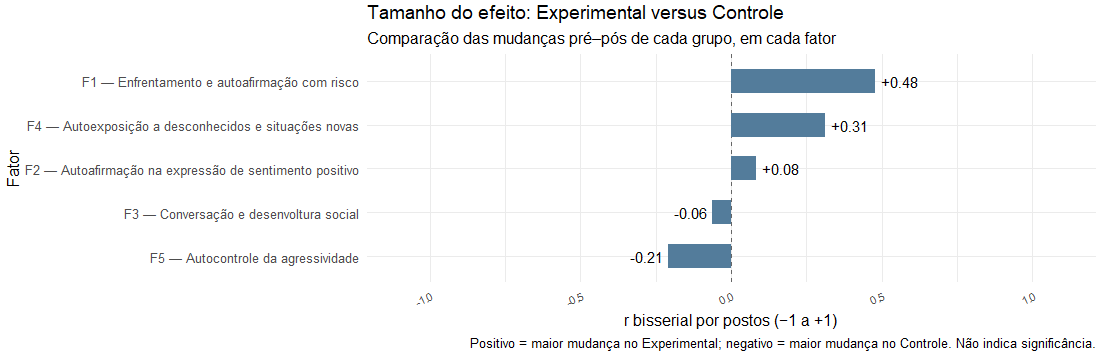
\includegraphics[width=1.3\linewidth]{imgs/tamanho_do_efeito.png}%
        }
        \caption{Tamanho do Efeito entre Grupos Experimental e Controle}
        \label{fig:tamanho_do_efeto}
        \par
        \vspace{2mm}
        \footnotesize Fonte: Próprio autor.
      \end{figure}



     Dessa forma, os resultados apontam diferenças descritivas favoráveis ao grupo experimental em quatro dos cinco fatores avaliados, especialmente em F1 e F4, como visto na Figura \ref{fig:mudancas_fatores}. Entretanto, essas diferenças \textbf{não foram estatisticamente significativas}, impossibilitando afirmar categoricamente que a participação nas sessões experimentais tenha produzido mudanças superiores às observadas no grupo controle.

     \begin{figure}[htbp]
        \centering
        \makebox[\linewidth][c]{%
          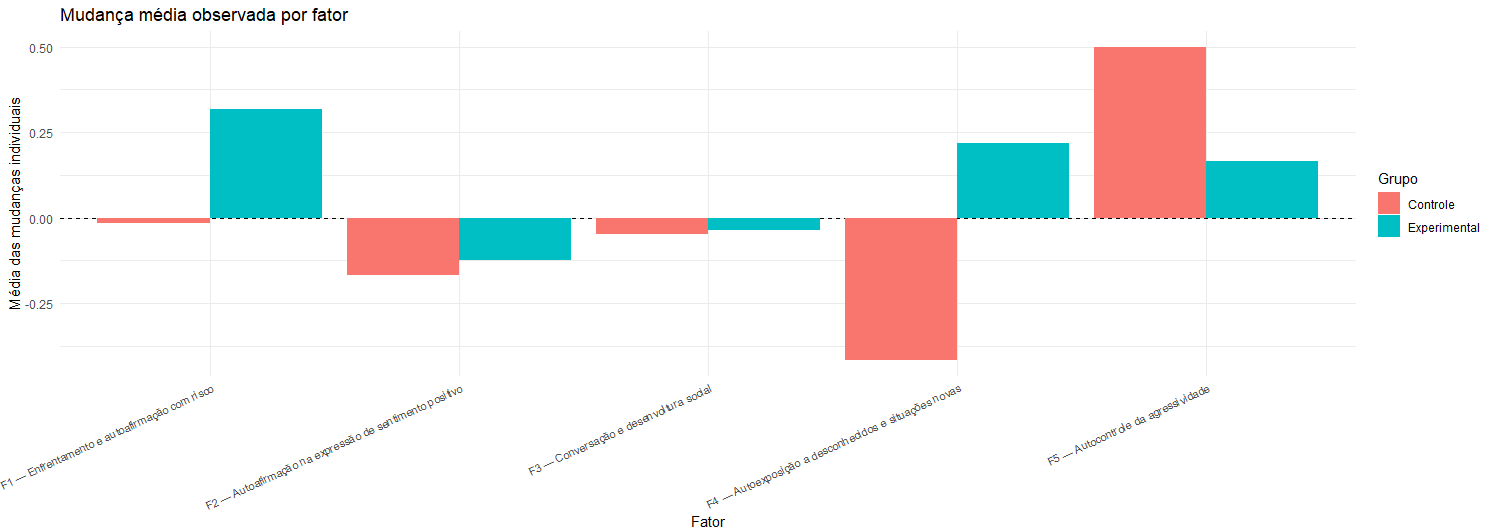
\includegraphics[width=1.3\linewidth]{imgs/06_mudancas_fatores.png}%
        }
        \caption{Mudança média nos cinco fatores do IHS entre os grupos experimental e controle.}
        \label{fig:mudancas_fatores}
        \par
        \vspace{2mm}
        \footnotesize Fonte: Próprio autor.
      \end{figure}


    \subsection{Análises individuais das mudanças nos fatores IHS}

      \subsubsection{Análise geral}
        Com o objetivo de investigar as variações individuais nas habilidades sociais dos voluntários, foi realizada uma análise descritiva das diferenças entre os resultados pré e pós-experimento para os cinco fatores do IHS. Para cada voluntário, foi calculada a diferença entre os indicadores dos dois momentos ($\Delta = \text{Pós} - \text{Pré}$), permitindo identificar aumentos, reduções ou ausências de mudanças em cada uma das dimensões avaliadas.

        Os resultados foram organizados em um mapa de calor, apresentado na Figura \ref{fig:heatmap_individual}, no qual as linhas representam os voluntários, agrupados entre experimental e controle, e as colunas correspondem aos cinco fatores. As tonalidades verdes representam aumentos nos indicadores, as vermelhas indicam reduções e as brancas representam ausência de mudança. A intensidade das cores corresponde à magnitude das diferenças observadas.

        \begin{figure}[!]
          \centering
          \makebox[\textwidth][c]{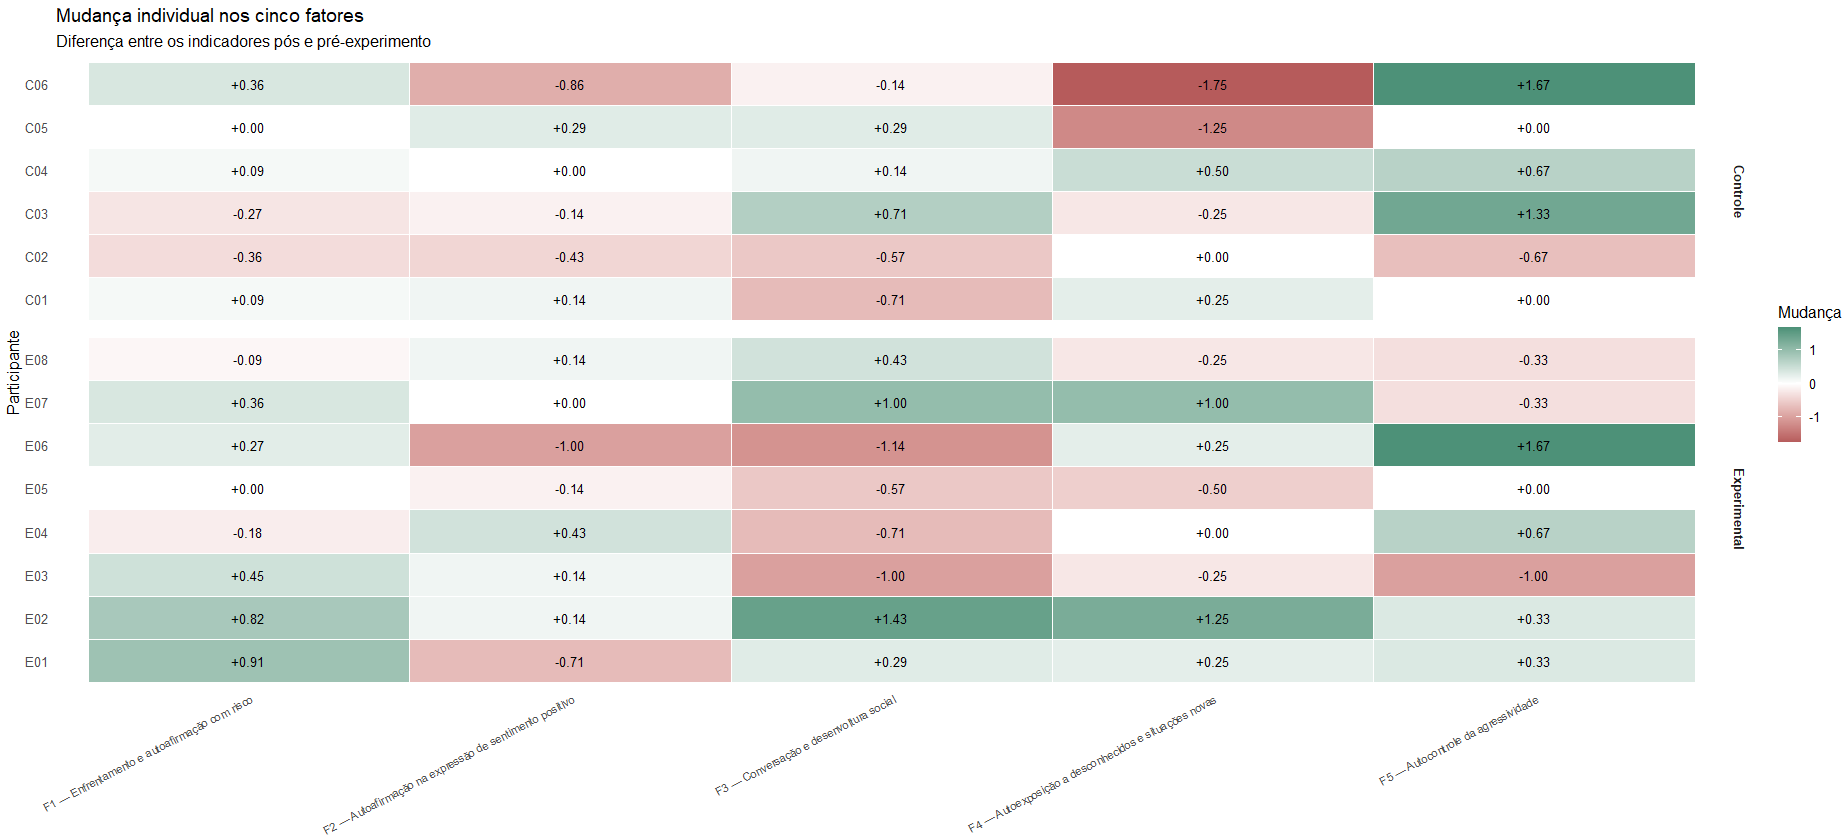
\includegraphics[width=1.5\textwidth]{imgs/04_mapa_calor_individual.png}}
          \caption{Mudanças individuais nos cinco fatores do IHS entre os momentos pré e pós-experimento.}
          \label{fig:heatmap_individual}
          \vspace{2mm}
          \begin{minipage}{\textwidth}
          \footnotesize
          \textit{Nota:}
          E01--E08 = voluntários do grupo experimental;
          C01--C06 = voluntários do grupo controle;
          F1 = Enfrentamento e autoafirmação com risco;
          F2 = Autoafirmação na expressão de sentimento positivo;
          F3 = Conversação e desenvoltura social;
          F4 = Autoexposição a desconhecidos e situações novas;
          F5 = Autocontrole da agressividade;
          Valores positivos indicam aumento no indicador, negativos indicam redução e zero indica ausência de mudança.
          \end{minipage}
          \par
          \vspace{2mm}
          \footnotesize Fonte: Próprio autor.
        \end{figure}


        A análise individual revelou considerável heterogeneidade nas mudanças apresentadas pelos voluntários. No grupo experimental, destacaram-se os voluntários E01 e E02, que apresentaram aumentos em quatro dos cinco fatores avaliados. O voluntário E02 apresentou aumentos expressivos em F1 (\textbf{+0,82}), F3 (\textbf{+1,43}) e F4 (\textbf{+1,25}), enquanto E01 apresentou seu maior aumento em F1 (\textbf{+0,91}). Por outro lado, o voluntário E05 apresentou reduções em três fatores e ausência de mudança nos outros dois, evidenciando que os resultados não foram uniformes entre os voluntários do experimento.

        Outros voluntários do grupo experimental apresentaram resultados mistos. O voluntário E06, por exemplo, registrou aumento em F5 (\textbf{+1,67}), mas reduções em F2 (\textbf{-1,00}) e F3 (\textbf{-1,14}). Já E07 apresentou aumentos em F3 (\textbf{+1,00}) e F4 (\textbf{+1,00}), acompanhados de uma pequena redução em F5 (\textbf{-0,33}). Esses resultados demonstram que um mesmo voluntário pode apresentar mudanças em direções diferentes, dependendo da dimensão de habilidade social analisada.

        No grupo controle, também foram observadas variações individuais. O voluntário C03 apresentou aumentos em F3 (\textbf{+0,71}) e F5 (\textbf{+1,33}), enquanto C06 apresentou aumento expressivo em F5 (\textbf{+1,67}), acompanhado de reduções em F2 (\textbf{-0,86}) e F4 (\textbf{-1,75}). O voluntário C02, por sua vez, apresentou reduções em quatro fatores e ausência de mudança em F4.

        De maneira geral, os resultados evidenciam que as mudanças nas habilidades sociais não ocorreram de forma homogênea, tanto no grupo experimental quanto no controle. Embora alguns voluntários do grupo experimental tenham apresentado aumentos em múltiplos fatores, outros registraram reduções ou resultados mistos. Além disso, a presença de aumentos e reduções expressivos no grupo controle demonstra que variações individuais também ocorreram independentemente da participação nas sessões experimentais. No entanto, é importante afirmar que, quando apresentada a pergunta "Você participou de algum evento ou situação na qual pode ter influenciado suas interações sociais fora do experimento?", apenas C4 respondeu que não, o que pode ter influenciado os resultados individuais (está melhor detalhado na análise descritiva, na Seção \ref{analisedescritiva}.

      \subsubsection{Comparação por participação}
        Com o objetivo de explorar a relação entre a frequência de participação nas sessões experimentais e as mudanças nas habilidades sociais, foi realizada uma análise descritiva. A Figura \ref{fig:mudancas_fatoresf1} apresenta os resultados do fator F1 (Enfrentamento e autoafirmação com risco), enquanto a Figura \ref{fig:mudancas_fatoresf4} apresenta os resultados do fator F4 (Autoexposição a desconhecidos e situações novas), selecionados por apresentarem os maiores tamanhos de efeito favoráveis ao grupo experimental.
        \begin{figure}[htbp]
          \centering
          \makebox[\linewidth][c]{%
          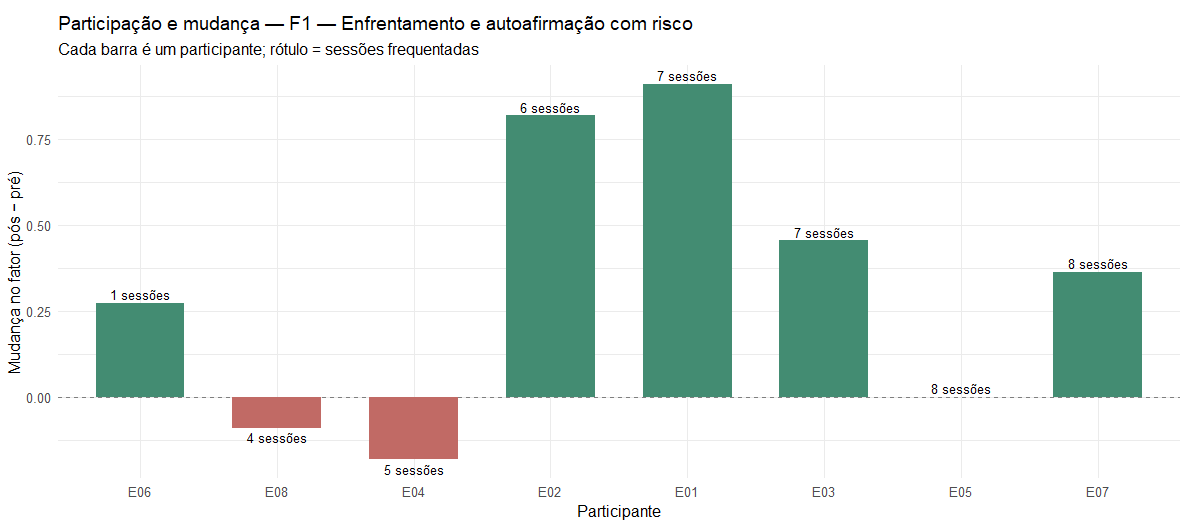
\includegraphics[width=1.3\linewidth]{imgs/f1-por-sesão.png}%
        }
          \caption{Enfrentamento e autoafirmação com risco (F1) por sessão}
          \label{fig:mudancas_fatoresf1}
          \par
          \vspace{2mm}
          \footnotesize Fonte: Próprio autor.
        \end{figure}

        \begin{figure}[htbp]
          \centering
          \makebox[\linewidth][c]{%
          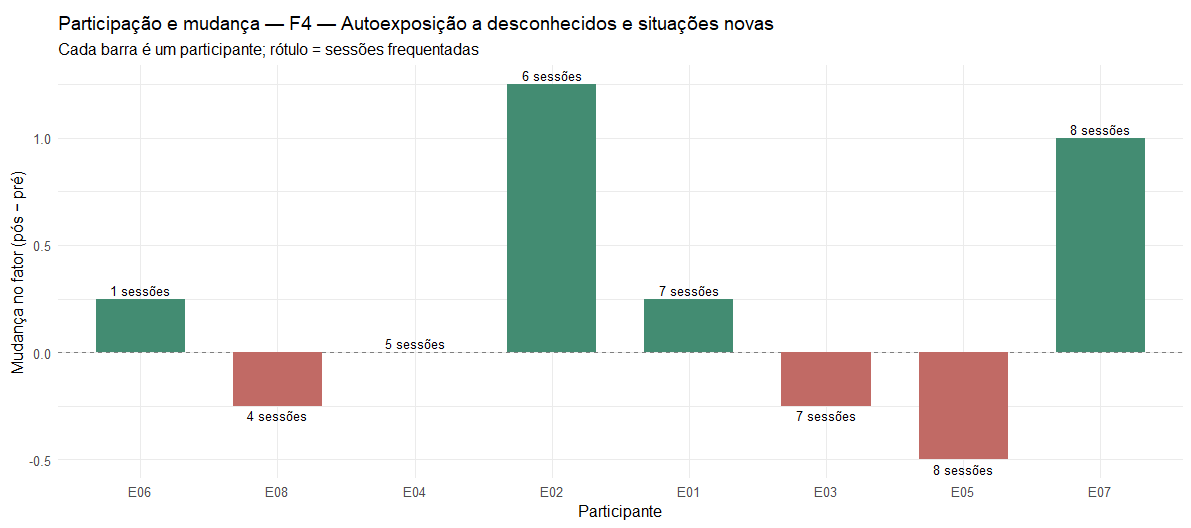
\includegraphics[width=1.3\linewidth]{imgs/f4-por-sesão.png}%
        }

          \caption{Autoexposição a desconhecidos e situações novas (F4) por sessão}
          \label{fig:mudancas_fatoresf4}
          \par
          \vspace{2mm}
          \footnotesize Fonte: Próprio autor.
        \end{figure}

        No fator F1, voluntários com maior frequência de sessões apresentaram, em sua maioria, aumentos nos indicadores. Já em F4, os resultados foram mais heterogêneos, com aumentos e reduções mesmo entre voluntários com frequência elevada. Assim, embora tenham sido observadas mudanças positivas em alguns voluntários, não foi identificado um padrão consistente entre o número de sessões frequentadas e a magnitude das mudanças.


  \section{Análise Descritiva}\label{analisedescritiva}
    \subsection{Dados pré-experimento}
        A amostra foi composta por 14 voluntários, distribuídos entre o grupo experimental (n = 8) e o grupo controle (n = 6). Conforme apresentado nas Figuras \ref{fig:demografia_experimental} e \ref{fig:demografia_controle}, o grupo experimental apresentou idades entre 18 e 28 anos, com predominância de voluntários do sexo masculino (4) e ensino superior incompleto (4). Já o grupo controle apresentou idades entre 17 e 27 anos, com predominância masculina (5) e ensino médio completo (3). Em ambos os grupos, observou-se uma concentração de voluntários jovens, com diferenças na distribuição por sexo e escolaridade.
        \begin{figure}[htbp]
          \centering
          \makebox[\linewidth][c]{
          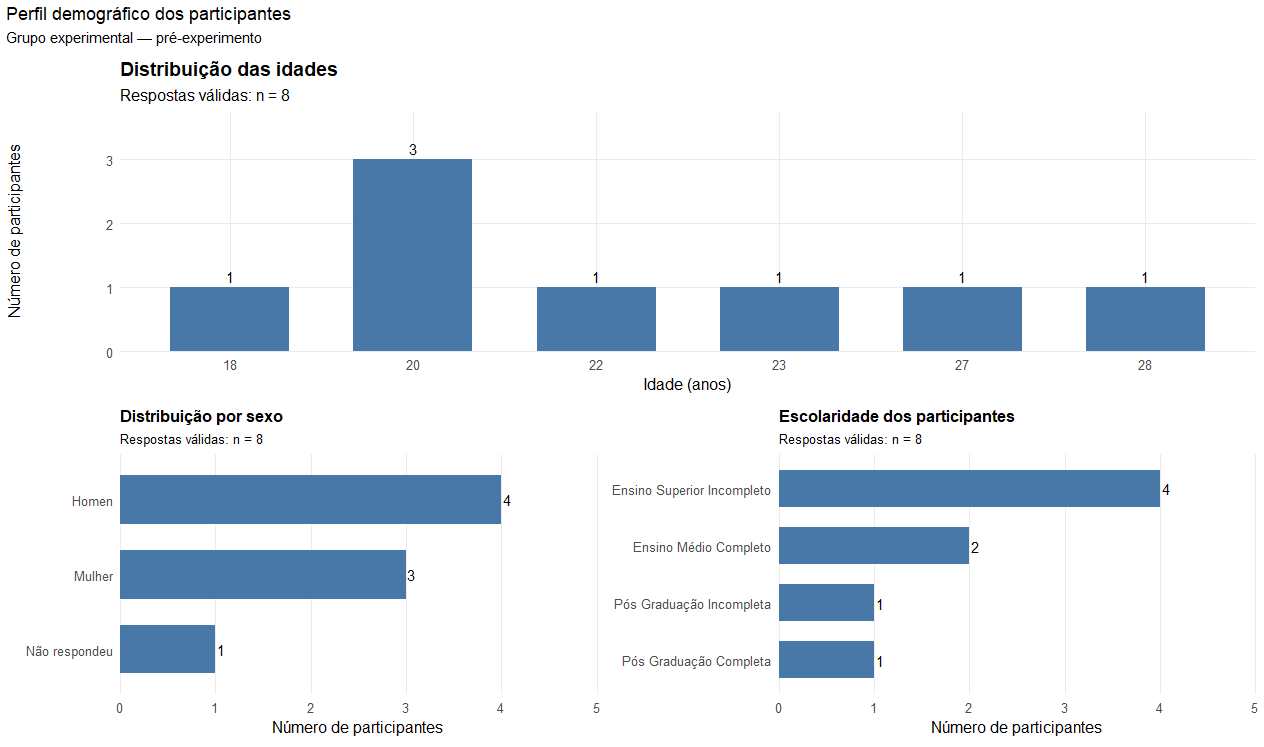
\includegraphics[width=1.3\linewidth]{imgs/dados_demograficos_ex.png}%
        }
          \caption{Perfil demográfico dos voluntários do grupo experimental (n = 8), considerando idade, sexo e escolaridade.}
          \label{fig:demografia_experimental}
          \par
          \vspace{2mm}
          \footnotesize Fonte: Próprio autor.
        \end{figure}

        % Figura — Perfil demográfico do grupo controle
        \begin{figure}[htbp]
          \centering
          \makebox[\linewidth][c]{%
          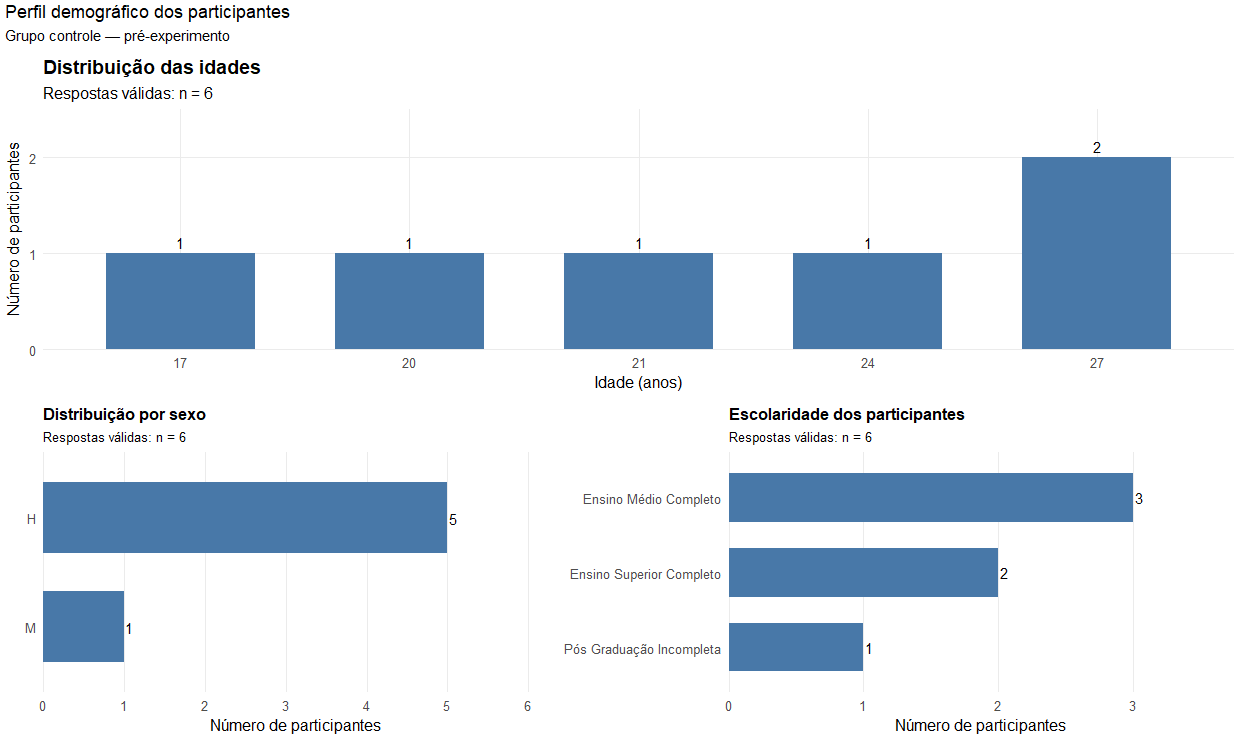
\includegraphics[width=1.3\linewidth]{imgs/dados_demograficos_co.png}%
        }
          \caption{Perfil demográfico dos voluntários do grupo controle (n = 6), considerando idade, sexo e escolaridade.}
          \label{fig:demografia_controle}
          \par
          \vspace{2mm}
          \footnotesize Fonte: Próprio autor.
        \end{figure}

        Conforme apresentado na Figura \ref{fig:perfil_experiencia}, entre os oito voluntários do grupo experimental, quatro (50\%) declararam se considerar tímidos, enquanto os outros quatro (50\%) não se identificaram dessa forma. Em relação à experiência anterior com o jogo \textit{Among’Us}, sete voluntários (87,5\%) afirmaram já ter jogado, enquanto apenas um (12,5\%) não possuía experiência prévia. Esses resultados indicam que, embora os voluntários apresentassem diferentes percepções sobre sua timidez, a maioria já estava familiarizada com o jogo utilizado no experimento.
        % Figura — do perfil e experiencia
        \begin{figure}[htbp]
            \centering
            \makebox[\linewidth][c]{%
          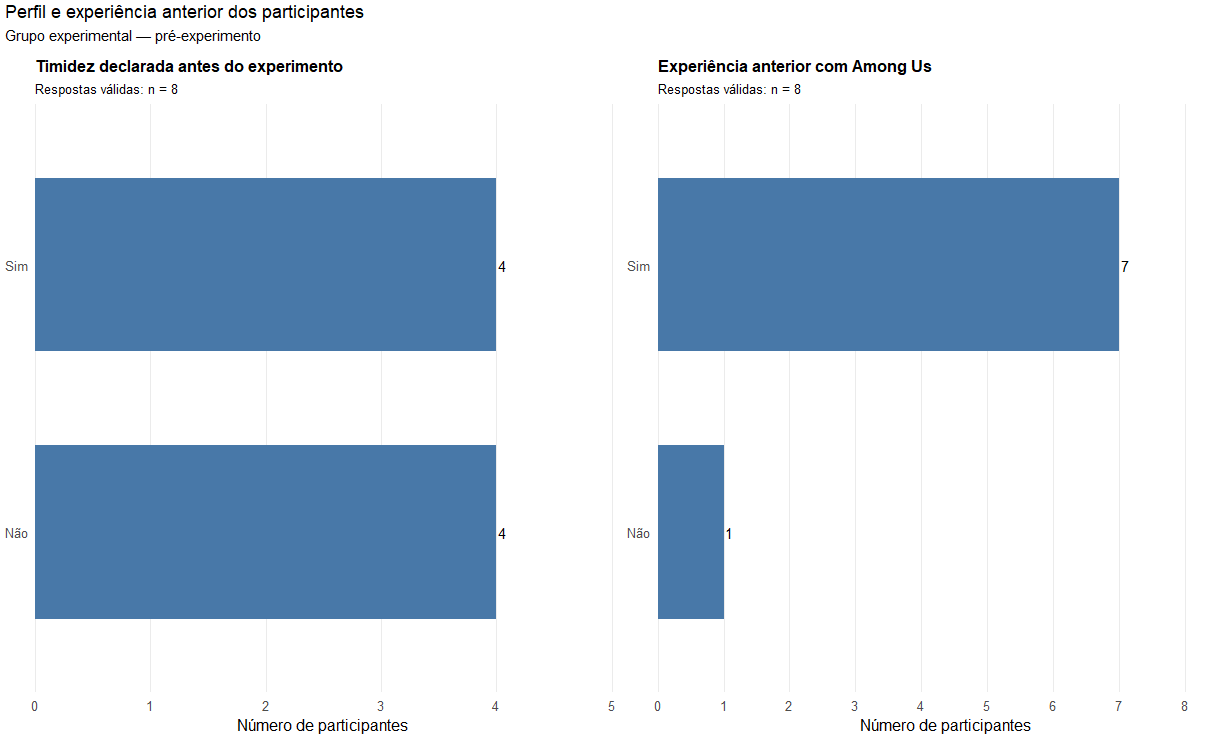
\includegraphics[width=1.3\linewidth]{imgs/timidez_e_experiencia.png}%
        }
            \caption{Timidez declarada e experiência anterior com Among’Us entre os voluntários do grupo experimental (n = 8).}
            \label{fig:perfil_experiencia}
            \par
            \vspace{2mm}
            \footnotesize Fonte: Próprio autor.
        \end{figure}


    \subsection{Dados pós-experimento}
      \subsubsection{Dados demográficos e aprovação do experimento}
        Conforme apresentado na Figura \ref{fig:sessoes_horarios}, a participação dos voluntários nas sessões experimentais variou entre uma e oito sessões. Dos oito voluntários, quatro (50\%) participaram de sete ou oito sessões, enquanto os demais apresentaram frequências de participação entre uma e seis sessões. Em relação à adequação dos horários estabelecidos, sete voluntários (87,5\%) consideraram os dias e horários apropriados, enquanto apenas um (12,5\%) manifestou insatisfação. Esses resultados indicam uma variação na frequência de participação, apesar da avaliação predominantemente positiva dos horários disponibilizados.
        \begin{figure}[htbp]
            \centering
            \makebox[\linewidth][c]{%
          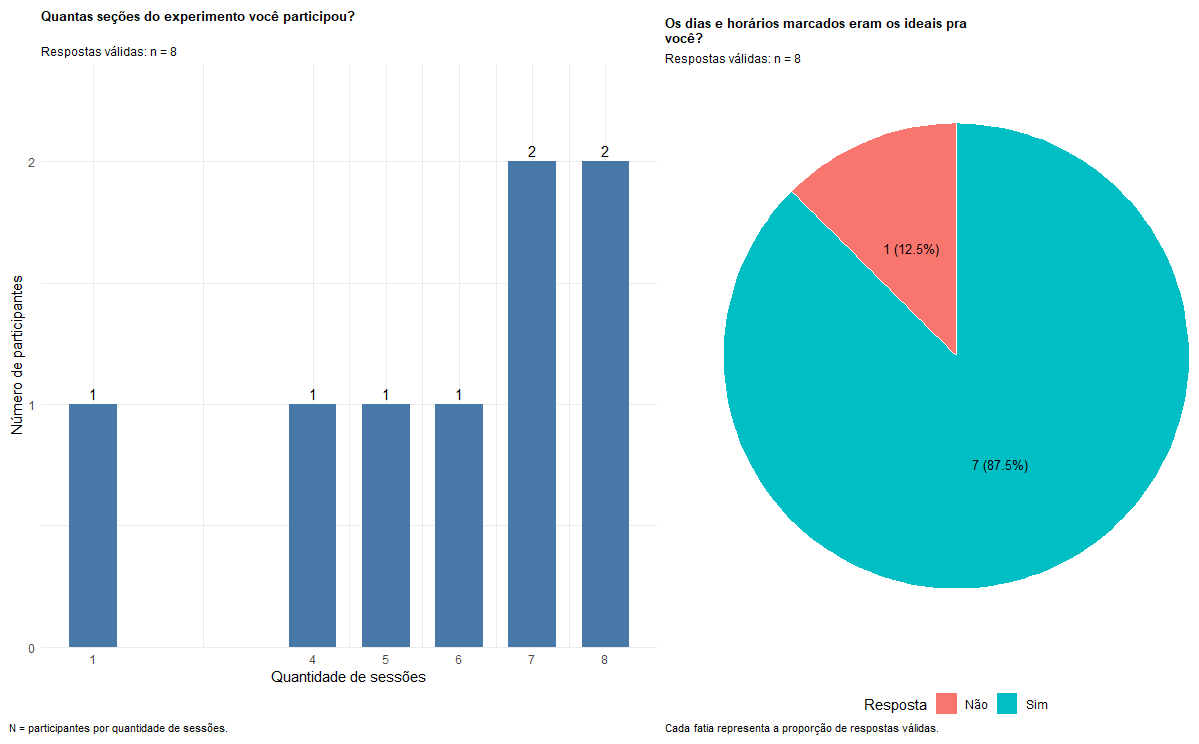
\includegraphics[width=1.3\linewidth]{imgs/sessões_e_horarios.png}%
        }
            \caption{Quantidade de sessões frequentadas pelos voluntários do grupo experimental e avaliação da adequação dos dias e horários estabelecidos (n = 8).}
            \label{fig:sessoes_horarios}
            \par
            \vspace{2mm}
            \footnotesize Fonte: Próprio autor.
        \end{figure}

        A avaliação da experiência dos voluntários durante o experimento apresentou resultados predominantemente positivos, conforme a Figura \ref{fig:diversao_geral}. Todos os voluntários atribuíram avaliações elevadas à diversão proporcionada pelas sessões, indicando uma boa receptividade à atividade proposta. Ao considerar os diferentes papéis desempenhados no jogo, apresentados na Figura \ref{fig:diversao_papeis}, observa-se que tanto a experiência como Tripulante quanto como Impostor foi avaliada positivamente. Entretanto, o papel de Tripulante apresentou maior concentração de avaliações máximas, enquanto o de Impostor demonstrou uma distribuição mais equilibrada entre as notas 4 e 5. De modo geral, esses resultados sugerem que a dinâmica do jogo foi bem recebida pelos voluntários, independentemente do papel desempenhado.

        % Figura — Diversão geral durante o experimento
        \begin{figure}[htbp]
            \centering
            \makebox[\linewidth][c]{%
          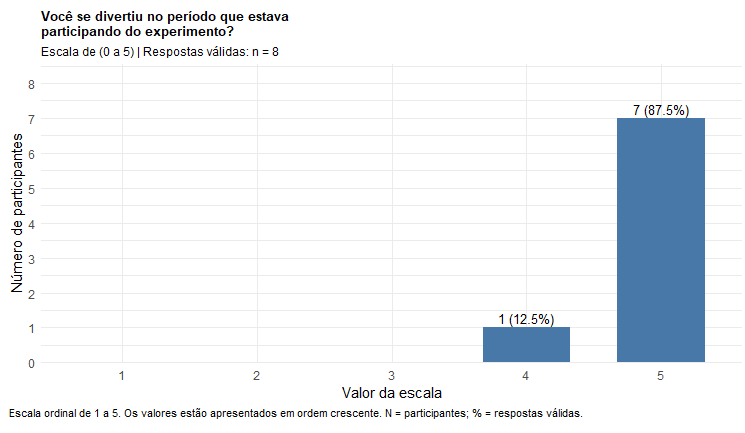
\includegraphics[width=1.0\linewidth]{imgs/divertiu.png}%
        }
            \caption{Avaliação da diversão geral durante as sessões experimentais, em escala de 0 a 5 (n = 8).}
            \label{fig:diversao_geral}
            \par
            \vspace{2mm}
            \footnotesize Fonte: Próprio autor.
        \end{figure}

        % Figura — Diversão por papel desempenhado
        \begin{figure}[htbp]
            \centering
            \makebox[\linewidth][c]{%
          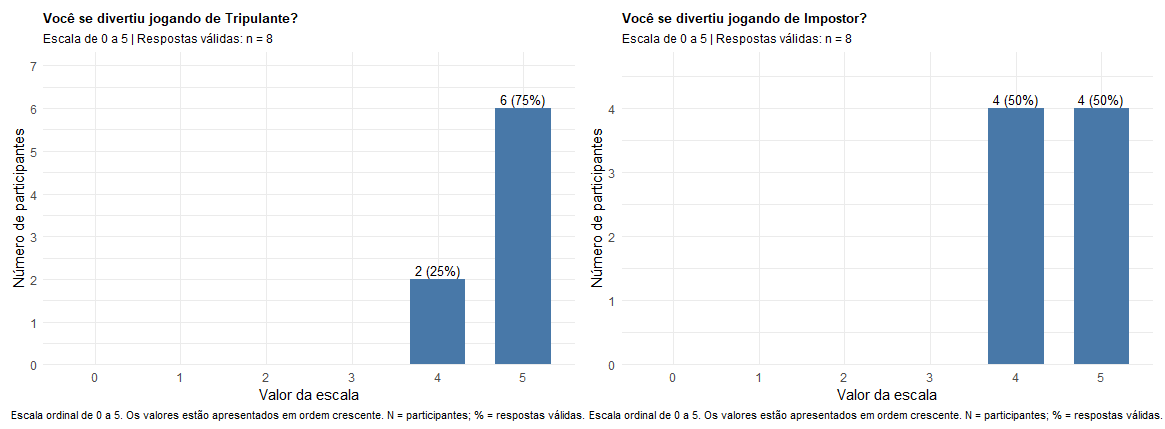
\includegraphics[width=1.3\linewidth]{imgs/tripulanteXimpostor.png}%
        }
            \caption{Avaliação da diversão dos voluntários ao desempenhar os papéis de Tripulante e Impostor, em escala de 0 a 5 (n = 8).}
            \label{fig:diversao_papeis}
            \par
            \vspace{2mm}
            \footnotesize Fonte: Próprio autor.
        \end{figure}

        \begin{figure}[htbp]
          \centering
          \makebox[\linewidth][c]{%
          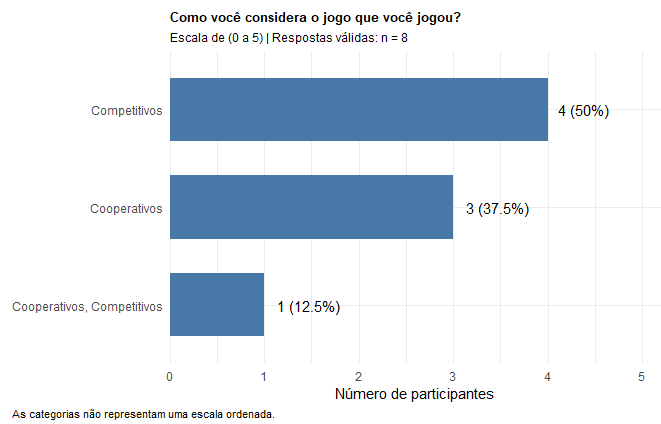
\includegraphics[width=1.3\linewidth]{imgs/cooperativoXcompetitivo.png}%
        }
          \caption{Percepção dos voluntários sobre o caráter cooperativo e competitivo do jogo Among’Us (n = 8).}
          \label{fig:avaliacao_jogo}
          \par
          \vspace{2mm}
          \footnotesize Fonte: Próprio autor.
        \end{figure}

        Em relação à percepção sobre a dinâmica do jogo, conforme apresentado na Figura \ref{fig:avaliacao_jogo}, os voluntários demonstraram diferentes interpretações, com predominância da classificação competitiva, seguida da cooperativa. Apenas um voluntário identificou o jogo como simultaneamente cooperativo e competitivo, evidenciando a presença de ambas as características na experiência dos jogadores.

      \subsubsection{Interação entre jogadores}
      A Figura \ref{fig:ajuda} apresenta a frequência com que os voluntários solicitavam e ofereciam ajuda durante as sessões. Observa-se que ambas as ações ocorreram com frequências variadas, com maior concentração de respostas nos valores intermediários da escala. O oferecimento de ajuda apresentou avaliações ligeiramente superiores às solicitações, sugerindo uma maior disposição dos voluntários em auxiliar outros jogadores do que em buscar auxílio, o que condiz com a experiência no jogo relatada na Figura \ref{fig:perfil_experiencia}.


      % Figura — Solicitação e oferecimento de ajuda
      \begin{figure}[htbp]
          \centering
          \makebox[\linewidth][c]{%
          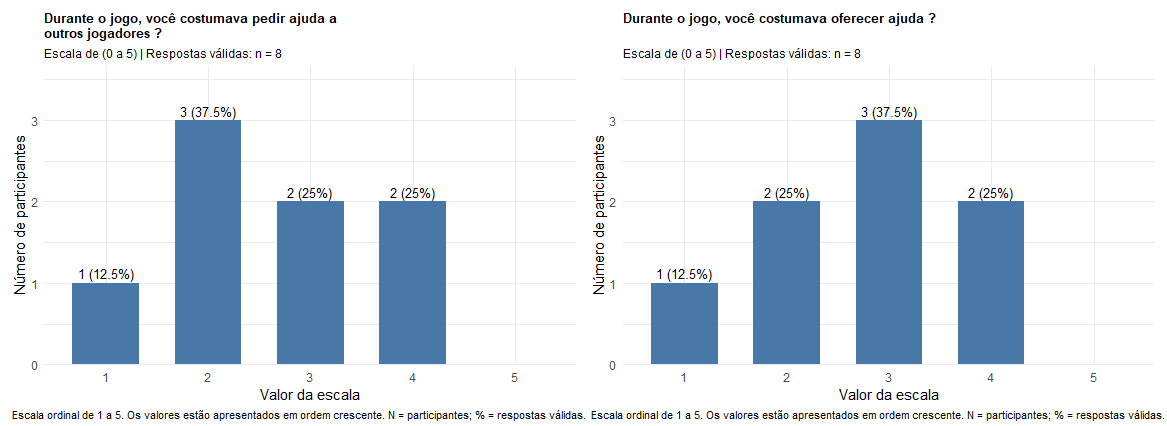
\includegraphics[width=1.3\linewidth]{imgs/ajuda.png}%
        }
          \caption{Frequência relatada de solicitação e oferecimento de ajuda durante as sessões experimentais, em escala de 0 a 5 (n = 8).}
          \label{fig:ajuda}
          \par
            \vspace{2mm}
            \footnotesize Fonte: Próprio autor.
      \end{figure}

      Em relação à comunicação, a Figura \ref{fig:conversa} demonstra que a maioria dos voluntários relatou iniciar conversas com frequência relativamente elevada durante as partidas. Por outro lado, as respostas relacionadas à troca de \textit{feedback} apresentaram maior dispersão, indicando diferenças individuais na frequência desse comportamento. Esses resultados sugerem que o ambiente do jogo favoreceu oportunidades de interação verbal, embora comportamentos específicos, como pedir ajuda e trocar \textit{feedback}, tenham ocorrido de maneira menos uniforme entre os voluntários.

      % Figura — Conversação e feedback
      \begin{figure}[htbp]
          \centering
          \makebox[\linewidth][c]{%
          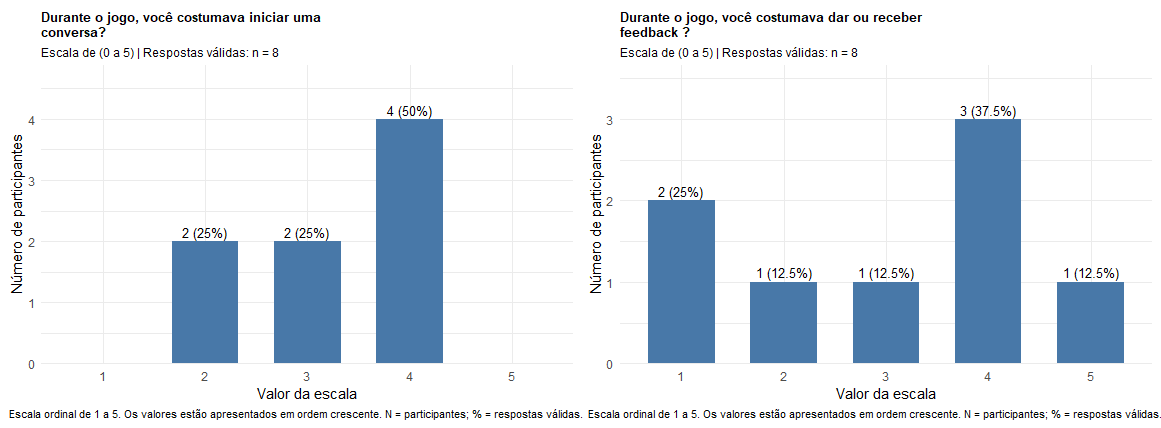
\includegraphics[width=1.3\linewidth]{imgs/conversa.png}%
        }
          \caption{Frequência relatada de início de conversas e troca de feedback durante as sessões experimentais, em escala de 0 a 5 (n = 8).}
          \label{fig:conversa}
          \par
            \vspace{2mm}
            \footnotesize Fonte: Próprio autor.
      \end{figure}

      \subsubsection{Desenvolvimento de Amizade}
        Em relação à socialização, a Figura \ref{fig:socializacao} demonstra que a maioria dos voluntários relatou maior conforto ao conversar com outras pessoas, enquanto todos afirmaram terem conhecido novas pessoas durante o experimento. Entretanto, metade relatou o desenvolvimento de novas amizades, sugerindo que as interações proporcionadas pelas sessões nem sempre resultaram na formação de vínculos mais próximos.

        % Figura — Socialização durante o experimento
        \begin{figure}[htbp]
            \centering
            \makebox[\linewidth][c]{%
            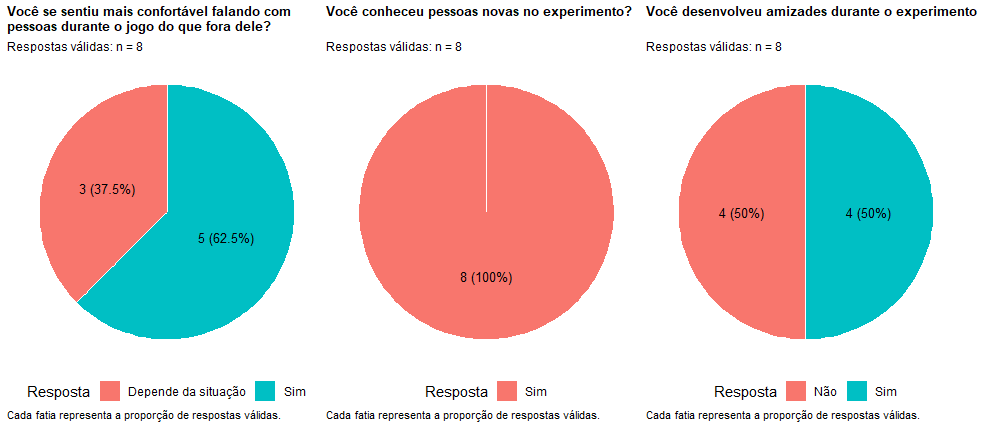
\includegraphics[width=1.3\linewidth]{imgs/amizades.png}%
          }
            \caption{Percepção dos voluntários sobre conforto nas interações sociais, conhecimento de novas pessoas e desenvolvimento de amizades durante o experimento (n = 8).}
            \label{fig:socializacao}
            \par
            \vspace{2mm}
            \footnotesize Fonte: Próprio autor.
        \end{figure}

        Além disso, conforme apresentado na Figura \ref{fig:conversas_diversas}, metade dos voluntários afirmou não ter conversado sobre assuntos externos ao experimento, enquanto os demais relataram essas conversas ou demonstraram incerteza. Esses resultados indicam que, embora o experimento tenha proporcionado oportunidades de socialização, as interações não necessariamente ultrapassaram o contexto das atividades propostas.

        % Figura — Conversas sobre assuntos externos ao experimento
        \begin{figure}[htbp]
            \centering
            \makebox[\linewidth][c]{%
            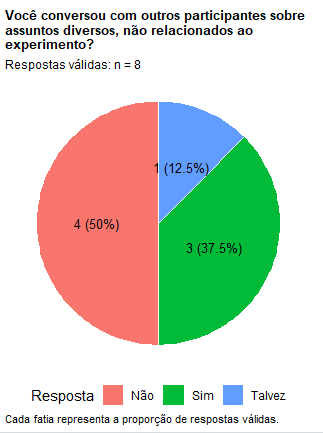
\includegraphics[width=0.5\linewidth]{imgs/fora_experimento.png}%
          }
            \caption{Relatos de conversas entre voluntários sobre assuntos não relacionados ao experimento (n = 8).}
            \label{fig:conversas_diversas}
            \par
            \vspace{2mm}
            \footnotesize Fonte: Próprio autor.
        \end{figure}

      \subsubsection{Autopercepção de desenvolvimento das habilidades sociais}
        Em relação à percepção de desenvolvimento das habilidades sociais, todos os voluntários do grupo experimental afirmaram ter percebido alguma melhora durante o período da pesquisa, conforme apresentado na Figura \ref{fig:desenvolvimento_percebido}. Esse resultado indica uma percepção subjetiva positiva da experiência, embora não represente, isoladamente, uma comprovação de desenvolvimento efetivo dessas habilidades.

        % Figura — Desenvolvimento percebido das habilidades sociais
        \begin{figure}[htbp]
            \centering
            \makebox[\linewidth][c]{%
            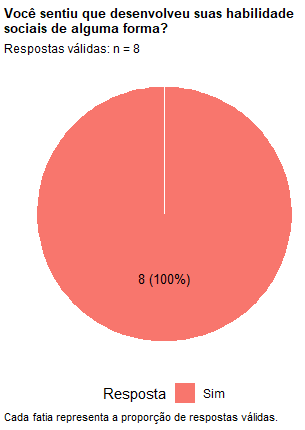
\includegraphics[width=0.4\linewidth]{imgs/seuntiu_hs.png}%
          }
            \caption{Percepção dos voluntários sobre o desenvolvimento de suas habilidades sociais durante o experimento (n = 8).}
            \label{fig:desenvolvimento_percebido}
            \par
            \vspace{2mm}
            \footnotesize Fonte: Próprio autor.
        \end{figure}



        Quanto à duração do experimento, apresentada na Figura \ref{fig:duracao_experimento}, as opiniões ficaram divididas entre considerar os dois meses adequados ou insuficientes. Entretanto, a maioria avaliou positivamente a duração individual das sessões de uma hora, sugerindo que uma possível ampliação do experimento poderia ocorrer pelo aumento do período total, sem necessariamente modificar a duração de cada sessão.

        % Figura — Avaliação da duração do experimento
        \begin{figure}[htbp]
            \centering
            \makebox[\linewidth][c]{%
            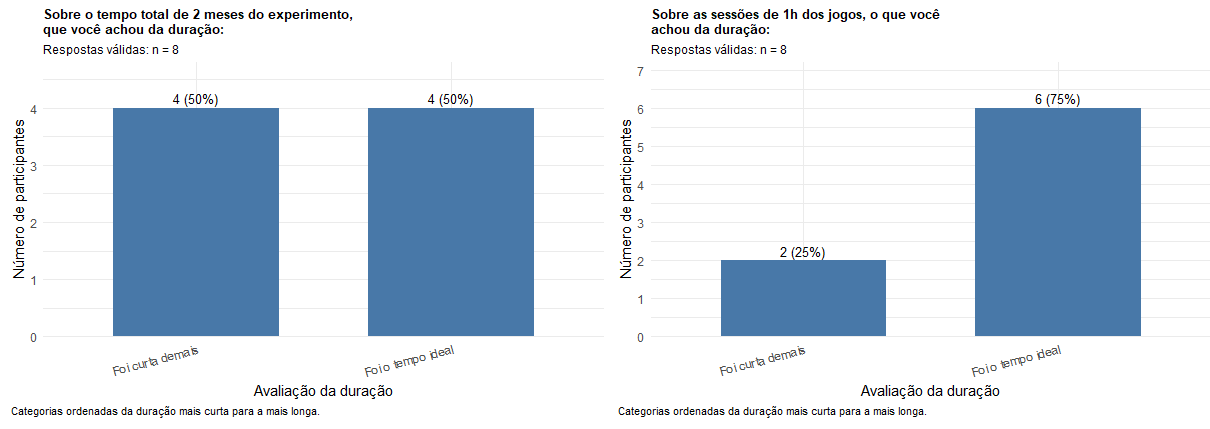
\includegraphics[width=1.3\linewidth]{imgs/tempo_de_experimento.png}%
          }
            \caption{Avaliação dos voluntários sobre a duração total de dois meses do experimento e a duração individual das sessões de uma hora (n = 8).}
            \label{fig:duracao_experimento}
            \par
            \vspace{2mm}
            \footnotesize Fonte: Próprio autor.
        \end{figure}

        % Figura — Crença na influência dos jogos multiplayer
        \begin{figure}[htbp]
            \centering
            \makebox[\linewidth][c]{%
            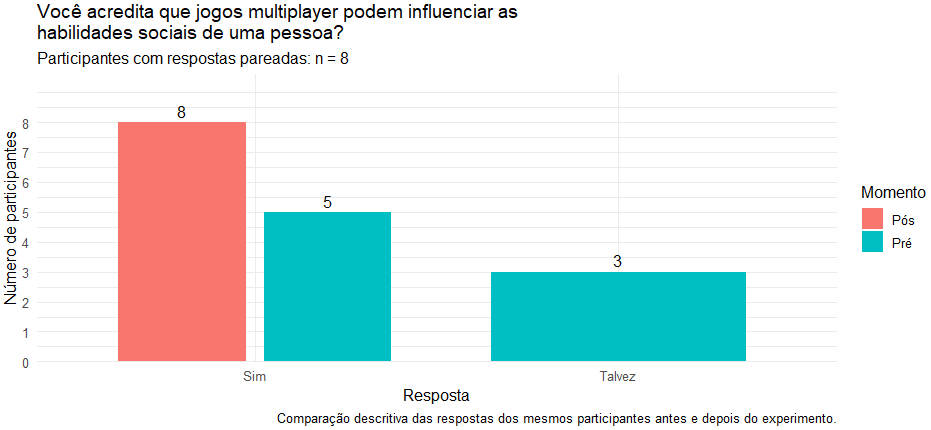
\includegraphics[width=1.3\linewidth]{imgs/acredita.png}%
          }
            \caption{Comparação das percepções dos voluntários sobre a influência dos jogos multiplayer nas habilidades sociais antes e após o experimento (n = 8).}
            \label{fig:crenca_multiplayer}
            \par
            \vspace{2mm}
            \footnotesize Fonte: Próprio autor.
        \end{figure}
        Por sua vez, a Figura \ref{fig:crenca_multiplayer} apresenta uma mudança na percepção dos voluntários sobre a influência dos jogos \textit{multiplayer} nas habilidades sociais. Antes do experimento, cinco voluntários acreditavam nessa influência, enquanto três demonstravam incerteza. Após a intervenção, todos passaram a acreditar que jogos \textit{multiplayer} podem influenciar as habilidades sociais, indicando uma mudança positiva na percepção dos voluntários sobre o potencial social desses jogos.


        \begin{figure}[htbp]
            \centering
            \makebox[\linewidth][c]{%
            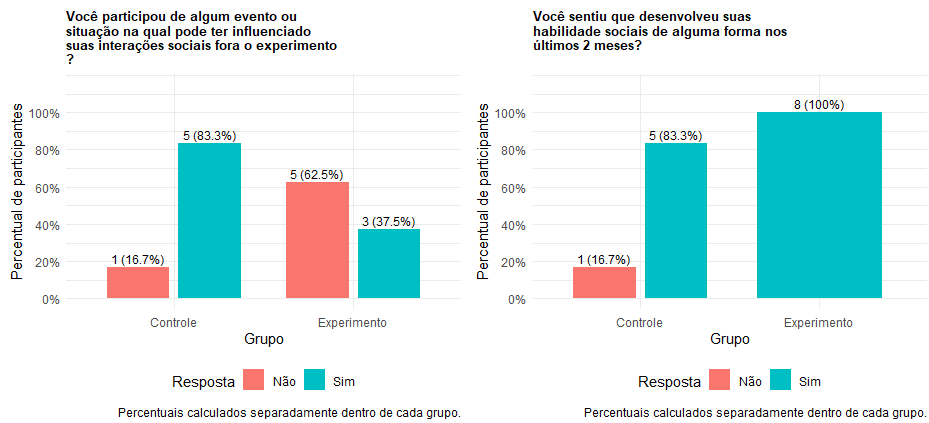
\includegraphics[width=1.3\linewidth]{imgs/comparativo.png}%
          }
            \caption{Comparação entre os grupos experimental (n = 8) e controle (n = 6) quanto à ocorrência de eventos externos que poderiam influenciar as interações sociais e à percepção de desenvolvimento das habilidades sociais nos últimos dois meses.}
            \label{fig:comparacao_grupos}
            \par
            \vspace{2mm}
            \footnotesize Fonte: Próprio autor.
        \end{figure}

        A Figura \ref{fig:comparacao_grupos} apresenta a comparação entre os grupos experimental e controle quanto à ocorrência de eventos externos e à percepção de desenvolvimento das habilidades sociais. Observa-se que a maioria dos voluntários do grupo controle relatou ter vivenciado situações externas que poderiam influenciar suas interações sociais, enquanto essa proporção foi menor no grupo experimental. Em relação ao desenvolvimento percebido, ambos os grupos apresentaram avaliações predominantemente positivas, com todos os voluntários do grupo experimental relatando  melhora. Esses resultados indicam que a percepção de desenvolvimento das habilidades sociais não foi exclusiva dos voluntários da intervenção, destacando a importância de considerar possíveis influências externas na interpretação dos resultados.